% arara: pdflatex: { shell: yes }
\documentclass[twoside]{article}
\usepackage[utf8]{inputenc}
\usepackage[english]{babel}
\usepackage{amsmath, amssymb, amsthm}
\usepackage{hyperref}
\usepackage{ragged2e}
\usepackage{graphicx}
\usepackage{float}
\usepackage{fancyhdr}
\usepackage{geometry}
\usepackage{multicol}
\usepackage{url}
\usepackage{listings} % For better code formatting
\usepackage{xcolor} % For syntax highlighting

% Suppress underfull and overfull warnings
\tolerance=1000
\emergencystretch=10pt

\setlength{\headheight}{15.2pt}
\geometry{paperwidth=8.5in, paperheight=11.0in, top=1.0in, bottom=1.0in, left=1.0in, right=1.0in}

\pagestyle{fancyplain}
\fancyhead[LO]{Activity \#3.1}
\fancyhead[CO]{}
\fancyhead[RO]{P25-LIS-3012}
\fancyfoot[LO]{\thepage}
\fancyfoot[CO]{Advanced Databases, UDLAP}
\fancyfoot[RO]{}

\begin{document}

\fancypagestyle{plain}{
  \renewcommand{\headrulewidth}{1pt}
  \renewcommand{\footrulewidth}{1pt}
}

\title{Lemmatization exercise}
\author{\small{Erick Gonzalez Parada ID: 178145}\\
  \small{Emiliano Ruiz Plancarte ID: 177478} \\
  \small{Andre Francois Duhamel Gutierrez ID: 177315} \\
\small{Antonio Gutiérrez Blanco ID: 177442}}
\date{\today}
\maketitle

\begin{abstract}
  \raggedright
  This document explores the implementation of a lemmatization system using the Snowball stemmer library to optimize text processing for search engines. By reducing words to their base forms and removing stop words, the system improves document retrieval efficiency. The integration of the Snowball stemmer into a Java application demonstrates its effectiveness in enhancing search engine performance.
\end{abstract}

\begin{justify}
  \textbf{\textit{Keywords:}} Stemmer , word, string, documents.
\end{justify}

\section{Characteristics of the problem}
\subsection*{Goals}
The primary goal of this project is to identify the limitations of a medium-level stemmer string processor and enhance its capabilities to be used as part of a future basic search engine. In document retrieval systems, optimization is critical, and all string processing must be as efficient as possible. The project focuses on improving the stemmer's ability to handle complex word structures, reduce words to their root forms, and remove stop words to enhance search engine performance.

\subsection*{Materials}
\begin{itemize}
  \item \textit{JDK 17 or above}
\end{itemize}

Text processing is a fundamental task in search engines, where efficiency and accuracy are critical for retrieving relevant documents. Traditional string processing methods often struggle with handling complex word structures, such as inflectional forms and stop words, which can degrade search engine performance \cite{geeksforgeeks1}. For example, words like "running," "ran," and "runs" should be reduced to their base form "run" to improve search accuracy. Additionally, stop words like "the," "and," and "or" add little semantic value but increase processing overhead \cite{geeksforgeeks3}. The Snowball stemmer, a widely used tool for lemmatization, addresses these challenges by reducing words to their root forms and removing stop words \cite{snowball}. However, integrating and optimizing such tools for specific applications, like search engines, requires careful customization and testing.

\section{Proposed Solution}
We, as a team, developed an improved version of the Snowball stemmer software, which is available at \url{https://github.com/HugeErick/Stemmer}. The solution involves the following steps:

\begin{itemize}
    \item \textbf{Refactoring the Snowball Stemmer}: The original Snowball stemmer code was refactored to integrate it into our Java application. This involved modifying the stemmer's API to handle English and Spanish text effectively.
    \item \textbf{Lemmatization and Stop Word Removal}: The application processes input text by reducing words to their root forms (lemmatization) and removing stop words (e.g., "the", "and", "or") to optimize search engine queries.
    \item \textbf{User Interaction}: The application allows users to input text and select the stemmer language (English or Spanish). The processed text is then displayed, showing the lemmatized output and the removed stop words.
    \item \textbf{Validation and Testing}: The system was tested with various text inputs to ensure accurate lemmatization and stop word removal. The results were validated against expected outputs to confirm the system's effectiveness.
\end{itemize}

The proposed solution demonstrates the successful integration of the Snowball stemmer into a Java application, providing a robust tool for text processing in search engine optimization.

\section{Interpretation of the findings} 
% result i.e screenshots of my program
% add interpretation to everything here

{\large proof that "snowball" was used}

\begin{figure}[H]
  \centering
  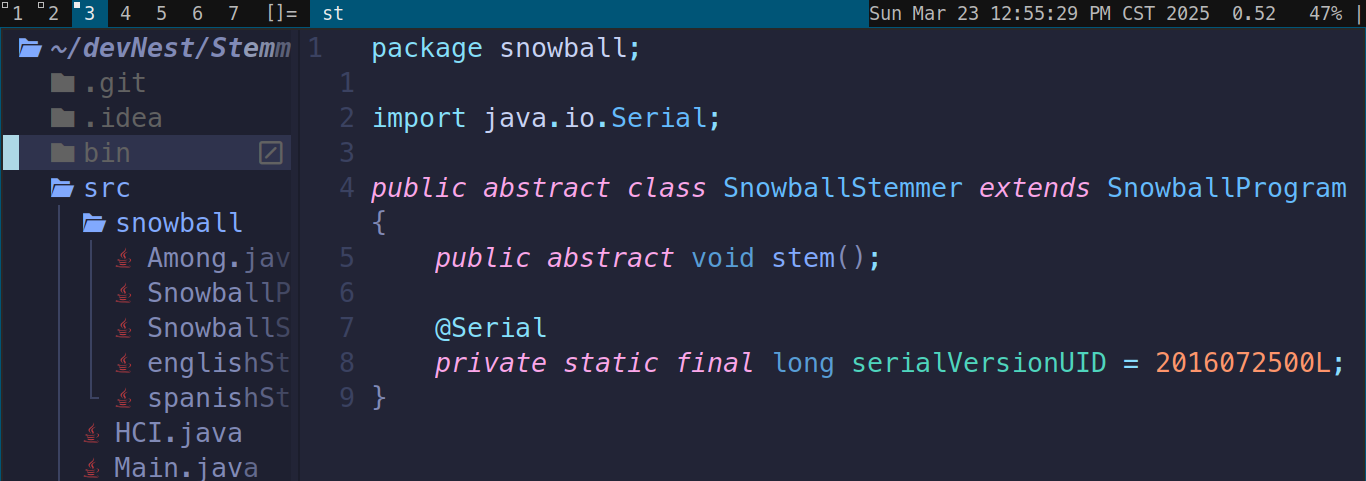
\includegraphics[width=1\textwidth]{imgs/proveSnow.png}
  \caption{The snowball software was refactored inside our program}
  \label{fig:1}
\end{figure}

The figure \ref{fig:1} shows that there was a severe refactorization of the code to be able to activate the API of the snowball. 

\begin{figure}[H]
  \centering
  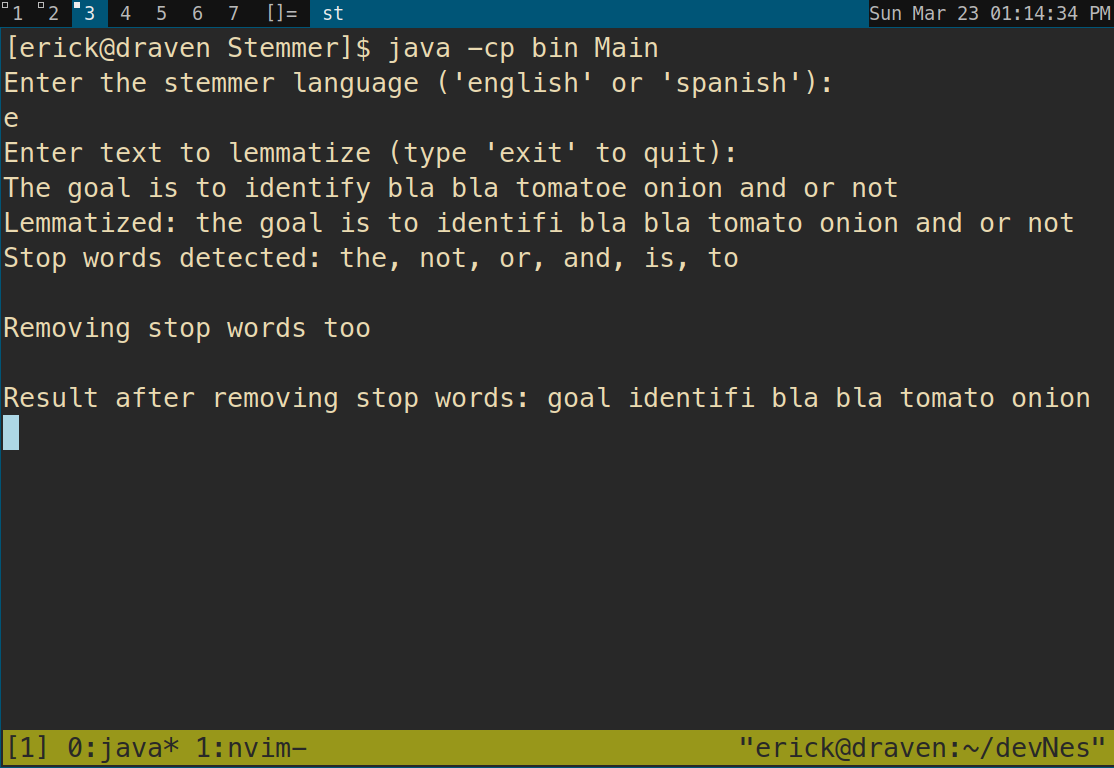
\includegraphics[width=1\textwidth]{imgs/use1.png}
  \caption{usage sample}
  \label{fig:2}
\end{figure}

The figure \ref{fig:2} shows a usage the example of the app

\begin{figure}[H]
  \centering
  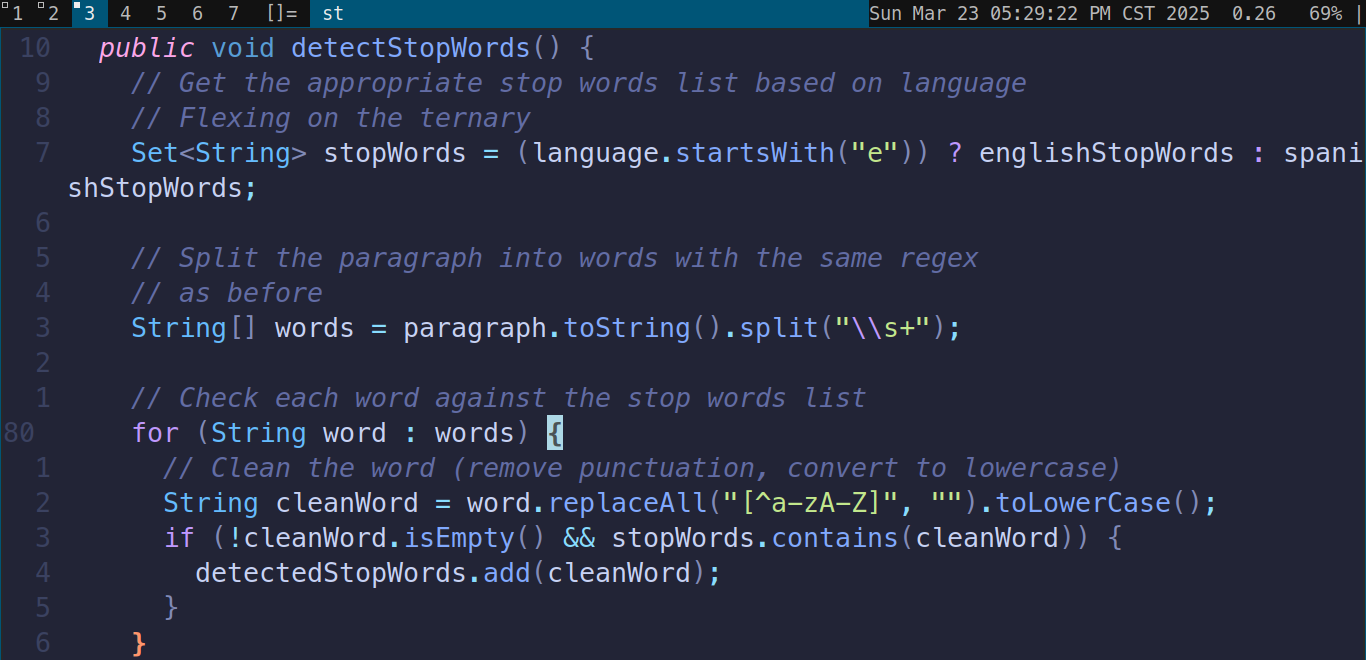
\includegraphics[width=1\textwidth]{imgs/stopWords.png}
  \caption{snapshot of some of the processing of the stop-words}
  \label{fig:3}
\end{figure}

The figure \ref{fig:3} shows a fragment of code where we are comparing the stemmed input against the stop words of the respective language\cite{geeksforgeeks2}.


\section{Access to Source Code}
The source code for this project is publicly available on GitHub at \url{https://github.com/HugeErick/Stemmer}. Anyone can access the repository to review the implementation, contribute to the project, or run the application locally. To get the application running, simply follow the instructions provided in the README file. The repository includes detailed steps for setting up the environment, compiling the code, and executing the application.

\section{Conclusions}
The project highlights the importance of efficient string processing in search engine optimization and demonstrates the successful use of the Snowball stemmer in achieving this goal.

\begin{thebibliography}{9}
  \bibitem{geeksforgeeks1}
  Applications, advantages and disadvantages of string. (2022, May 25). GeeksforGeeks. from \url{https://www.geeksforgeeks.org/applications-advantages-and-disadvantages-of-string/} 
  \bibitem{geeksforgeeks2}
  Gupta, M. (2016, November 11). Java StringTokenizer class. GeeksforGeeks. from \url{https://www.geeksforgeeks.org/stringtokenizer-class-in-java/} 
  \bibitem{geeksforgeeks3}
  Improve, G. (2017, July 10). How do search engines work? GeeksforGeeks. from \url{https://www.geeksforgeeks.org/search-engines-work/} 
  \bibitem{snowball}
  Snowball. (n.d.). Snowballstem.org. Retrieved March 23, 2025, from \url{https://snowballstem.org/}
\end{thebibliography}
\end{document}
